\documentclass{article}
\usepackage{ctex}
\usepackage[a4paper]{geometry}
\usepackage{amsthm,amsmath,amssymb}
\usepackage{ulem}
\usepackage{graphicx}
\usepackage{caption}
\usepackage{subcaption}
\usepackage{gensymb}
\usepackage{url}
\usepackage{hyperref}
\usepackage{enumitem}
\usepackage{color}

\begin{document}
\normalem
\section{Voronoi Treemaps\cite{Balzer2005}}
该论文提出的方法将treemap构成的基本元素从矩形拓展到了任形状,从而消除了一般treemap采用矩形时出现的横纵比不均衡以及不能清楚的展示数据的层次结构等问题。
所以Voronoi Treemap更具灵活性,能够在更多的应用中使用。
层次结构经常用作数据的分类、排序、组织的一种抽象,被广泛应用在多种数据中。
(Hierarchical structures are an often used abstraction for the classification, 
sorting, and organization of a broad variety of data.)
Treemap具有的space-efficiency特性,使得它被广泛应用在系谱图(family tree)、文件系统的组织结构、软件架构、
金融分析、体育报告等多种领域。

文章中的Voronoi Treemap的基础是centroidal voronoid tessellation\cite{du1999centroidal}的使用。这个技术被广泛应用在能量最小化的各个领域,比如
数据压缩,图像处理,网格细化(mesh refinement),资源分配以及科学可视化中。
\begin{figure}
  \centering
  \begin{subfigure}[h]{0.5\textwidth}
    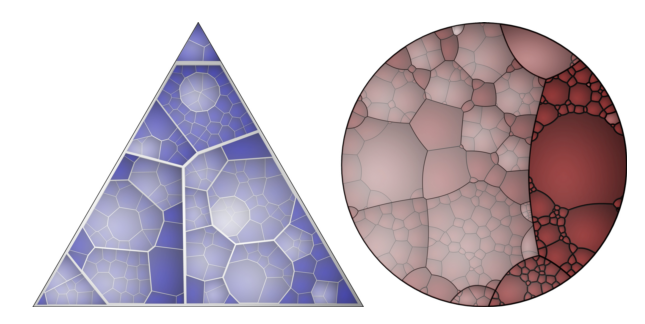
\includegraphics[width=0.8\textwidth]{_img/VoronoiTreemap_1.png}
    \label{fig:voronoi_treemap_1}
  \end{subfigure}

  \begin{subfigure}[h]{0.5\textwidth}
    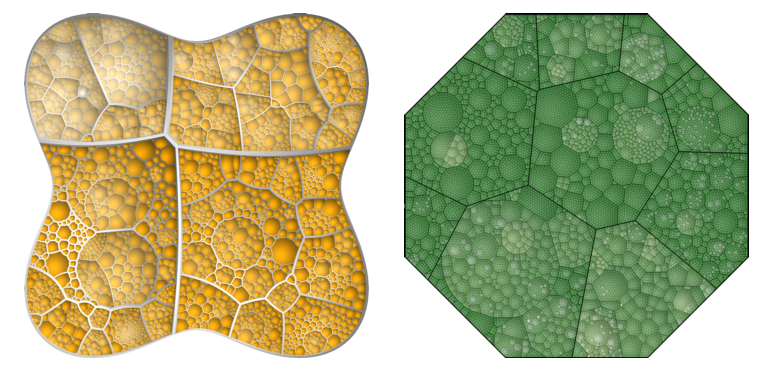
\includegraphics[width=0.8\textwidth]{_img/VoronoiTreemap_2.png}
    \label{fig:voronoi_treemap_1}
  \end{subfigure}
  \caption{Voronoi Treemap Examples}
\end{figure}

\section{Cheops: A Compact Explorer For Complex Hierarchies\cite{Beaudoin1996}}
数据量的增多,加大了层次数据可视化的难度,一方面数据越来越复杂,另一方面数据的节点一层一层呈指数增长。
一般的可视化技术能够有效的处理1000个几点左右的层次数据,一旦数据量超过5000,
就需要一些特殊的技术来弥补数据量过大造成的节点重叠等问题,比如通过cluster来减少节点数目,再通过交互方式显示被隐藏的节点。
但是cluster技术会影响可视结果的稳定性。

文章提出了一个浏览大量复杂层次数据的可视技术,Cheops,可以处理1000万到10亿的节点数目。
它能够在保持节点上下文环境的同时浏览节点的细节信息。

传统的方法一般是在基本的表现形式上通过交互来加强信息的显示,最常用的是focus+context和fisheye。
当这些方法用在比较复杂的数据上时会存在一些问题,
比如因为使用了DOI(Degree-of-Intrest)函数使得周围的节点扭曲。当焦点改变的时候有可能需要重绘整个视图,
效率就会有所下降。

\subsection{论文大意}
Cheops方法使用三角形作为可视的基本元素,通过元素重叠的方式节省空间,如图\ref{fig:Cheops_1}。
然后通过交互手段根据需要选择性的显示重叠的节点。在实际中节点并不是完全重叠。

\begin{figure}[h]
  \centering
  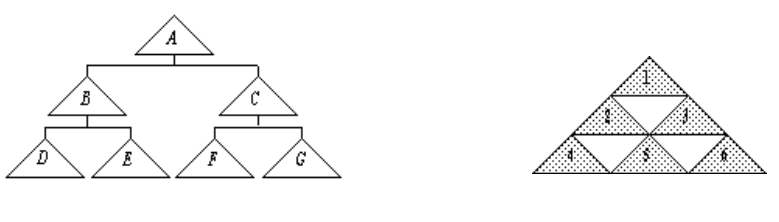
\includegraphics[width=0.8\textwidth]{_img/Cheops_1.png}
  \caption{从做图到右图的转换,左图中的EF两个节点在右图中重叠为节点5}
  \label{fig:Cheops_1}
\end{figure}

为了能够在动态的上下文中浏览节点,实现中使用了\emph{selecton}和\emph{pre-selection}技术。

\begin{itemize}
\item selection操作是说当用户选中一个节点(logical node)时,高亮显示以整个
  节点为根的树,其余的节点只显示一个轮廓如图\ref{fig:Cheops_2}左。旁边面板显示每个层次中选中的点的信息。
\item pre-selection是说用户选中一个节点后,随机的选择一个用户可能选择的子节
  点,用户通过鼠标操作可以在子节点中进行切换,如图\ref{fig:Cheops_2}右。
\end{itemize}

\begin{figure}[h]
  \centering
  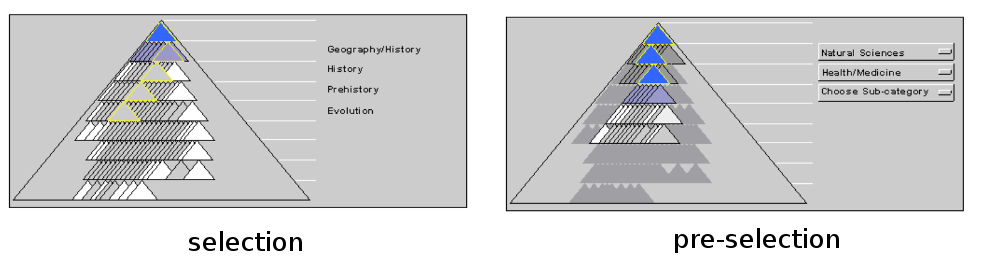
\includegraphics[width=0.8\textwidth]{_img/Cheops_2.png}
  \caption{selection和pre-selection}
  \label{fig:Cheops_2}
\end{figure}

这两种选择方式能够让用户在复杂的层次结构中快速的定位到节点。

另为除了在图上选择点以外,旁边面板提供的类似comb select的方式来选择节点,
图的下方也有navigation button来帮助用户选择。

其他的交互slider、bookmarks、histogram。
bookmarks允许用户保存某个视图,histogram用户显示节点或者当前选中结构的信息。
如图\ref{fig:Cheops_3}

\begin{figure}[h]
  \centering
  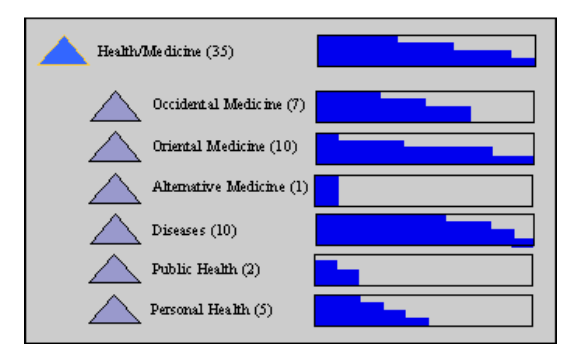
\includegraphics[width=0.8\textwidth]{_img/Cheops_3.png}
  \caption{图中可以看出,通过比较,disease节点应该是用户关注的下一个节点}
  \label{fig:Cheops_3}
\end{figure}

\subsection{缺点}

这个方法适合在大量数据中查找信息或者查看数据的结构特性。
在对数据属性的显示上呈现的效果不是很丰富,所以不适合用于数据的比较或者查看数据属性之间的关系。

\subsection{启发}

\begin{enumerate}
\item 交互中,同一个功能可能需要多种方式实现来方便不同用户或者在不同的状态下进行选择。
\item 交互不是目的,交互是为了方便用户提取图中的信息。
  所以可以以一种\emph{显示->交互->信息提取->显示->交互->信息提取}的循环模式逐步让用户提取信息。
\end{enumerate}

\subsection{思考}
overlap的方式在什么情况下适用?缺点?优点?

\bibliographystyle{plain}
\bibliography{ref_readings}
\end{document}
